\chapter{Analysis and Design of the Adaptive Fusion Framework}


\section{5.1 Introduction}


This chapter converts the conceptual approach described in Chapter 4 into a system-level design. The chapter focuses on architecture, data flow, component responsibilities, and the positioning of the adaptive fusion extension. In accordance with the thesis guideline, this chapter does not present implementation-level code or algorithmic details; those are discussed in Chapter 6.


\section{5.2 System Requirements and Assumptions}


The framework was designed to satisfy the following functional requirements:


1. Prepare a paired image-text fake news dataset with standardized labels.

2. Train and evaluate a separate image classification branch.

3. Train and evaluate a separate text classification branch.

4. Generate modality probabilities and confidence scores for train, validation, and test splits.

5. Estimate image and text reliability features.

6. Train an adaptive fusion controller that selects sample-level modality weights.

7. Compare the proposed fusion model with deterministic and supervised baselines.

8. Generate policy analysis, robustness analysis, and explainability artifacts.

9. Export thesis-ready result summaries.


The framework assumes that each final evaluation sample contains both text and an available image. It also assumes that training, validation, and test splits remain separate throughout the pipeline, with validation used for model selection and threshold tuning, and test used only for final evaluation.


\section{5.3 Top-Level Architecture}


The top-level architecture, shown in Figure 5.1, contains six major layers: data preparation, unimodal modelling, reliability construction, adaptive fusion, evaluation, and explainability. The data preparation layer standardizes raw Fakeddit metadata and creates train, validation, and test splits. The unimodal modelling layer contains the image and text branches. The reliability construction layer merges modality predictions with confidence and quality indicators. The adaptive fusion layer uses the reliability-aware state to select image-text weights. The evaluation layer compares results across baselines and proposed models. The explainability layer generates image, text, and fusion-level explanations.


The architecture is modular so that each stage can be tested and rerun independently. This is important because image downloading, GPU training, and evaluation can fail or require reruns in a cloud environment.


\section{5.4 Data Flow and Interaction Design}


The data flow begins with raw Fakeddit metadata files. These files are converted into a standard schema containing sample identifier, image path or URL, text, and label. A balanced final subset is created for computation. The image downloader attempts to obtain image files and then creates image-available splits containing only samples with successfully downloaded images.


After the final available splits are created, the image branch and text branch are trained separately. Each branch then produces prediction outputs for train, validation, and test data. These outputs are merged into reliability files. The fusion controller uses the train reliability file for learning, the validation reliability file for model selection, and the test reliability file for final evaluation.


The evaluation outputs are written as JSON and CSV files so that the thesis can cite file-backed evidence. The notebooks provide a human-readable execution record for demonstration and viva purposes.


\section{5.5 Design of Unimodal Branches}


The image branch is designed as a visual classifier that maps an input image to a binary probability. A residual convolutional architecture is used because it provides a strong general-purpose image representation. The output of the image branch is not only a predicted class but also a probability and confidence value.


The text branch is designed as a transformer-based classifier that maps cleaned text into a binary probability. It provides a text prediction, text probability, and text confidence. The text branch is kept separate from the image branch so that each modality can be evaluated independently before fusion.


This branch separation supports transparent evaluation. If the final fusion model improves over unimodal branches, the source of improvement can be examined through baseline and ablation results.


\section{5.6 Design of the Adaptive Fusion Controller}


The adaptive fusion controller is designed as the main research extension. It receives a compact reliability-aware state rather than raw image and text inputs. This state includes modality probabilities, confidence indicators, quality indicators, disagreement, and difference features. The controller selects a discrete fusion action, and each action maps to a specific pair of image and text weights.


This design makes fusion explainable because the selected action can be reported for each sample. The final prediction can therefore be explained in terms of the image branch probability, text branch probability, selected image weight, selected text weight, and final fused probability.


\section{5.7 Design of Baseline and Comparison Components}


The framework includes baseline components to make evaluation meaningful. Image-only and text-only baselines test the strength of each modality. Equal fusion and confidence-weighted fusion test simple decision-level multimodal fusion. Reliability-weighted fusion tests a deterministic use of reliability features. Supervised MLP fusion provides a learned non-RL comparison. These baselines are necessary because the proposed RL controller must be compared against simple and strong alternatives, not only against unimodal branches.


The comparison design also includes ablation experiments. Ablation allows the effect of state features to be analysed by comparing probabilities-only, prediction-confidence, and full reliability-aware states.


\section{5.8 Design of Explainability Outputs}


The explanation design has three levels. The image explanation uses a heatmap to indicate visually influential regions. The text explanation uses token saliency to indicate influential words or subword tokens. The fusion explanation records selected action, modality weights, and final probability.


This design is aligned with the research problem because the model is expected to explain not only what it predicted, but also how image and text evidence were combined.


\section{5.9 Summary}


This chapter described the system design of the adaptive fusion framework. The design separates data preparation, unimodal modelling, reliability construction, adaptive fusion, evaluation, and explainability into modular components. The next chapter explains how this design was implemented in the project repository.

\begin{figure}[H]
\centering
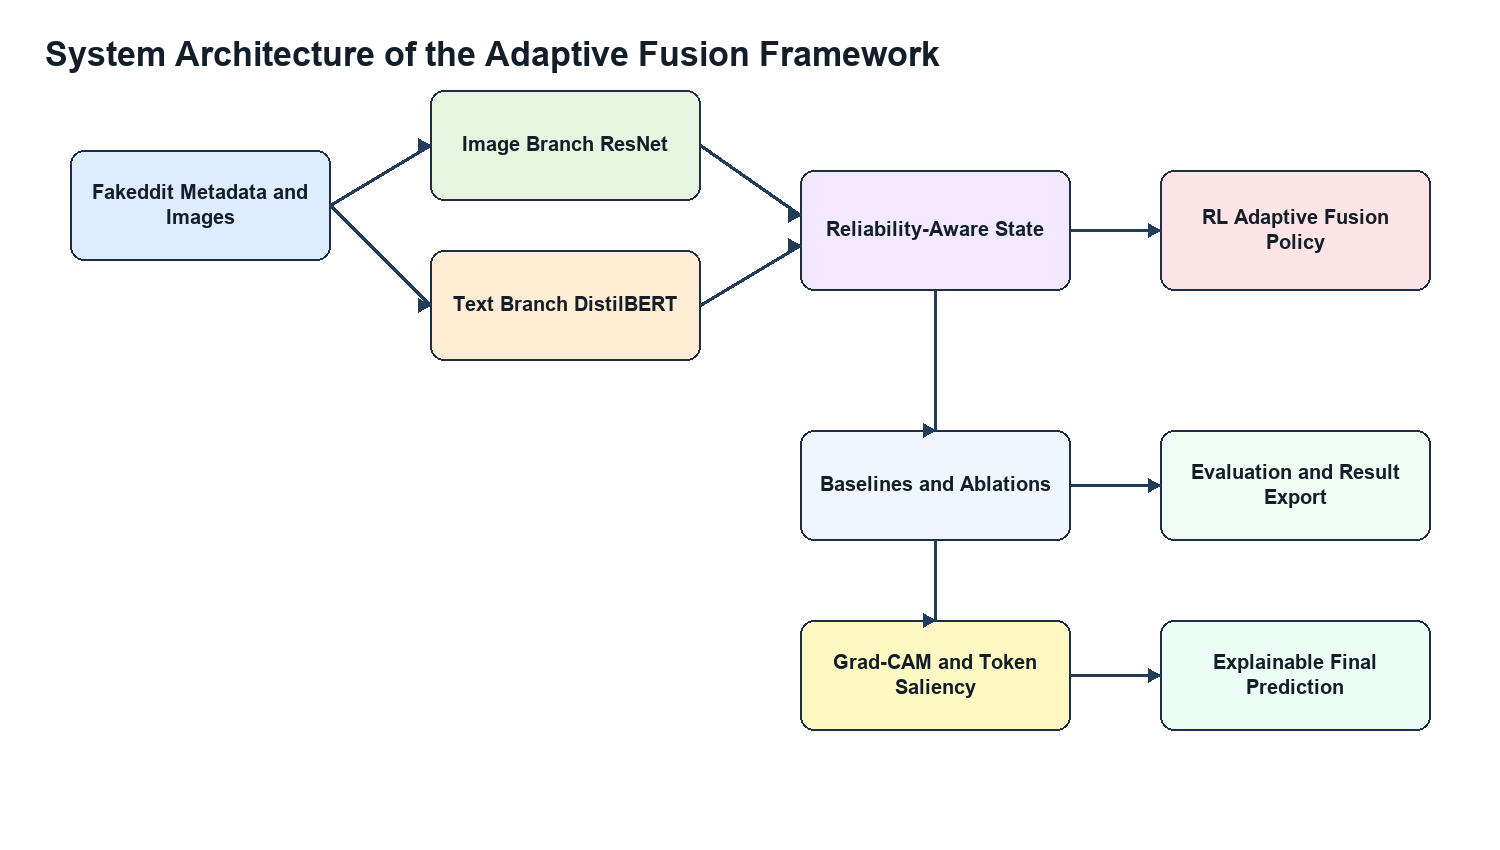
\includegraphics[width=0.92\textwidth,height=0.42\textheight,keepaspectratio]{figures/figure_5_1_system_architecture.png}
\caption{System architecture of the adaptive fusion framework.}
\label{fig:system_architecture}
\end{figure}

\begin{figure}[H]
\centering
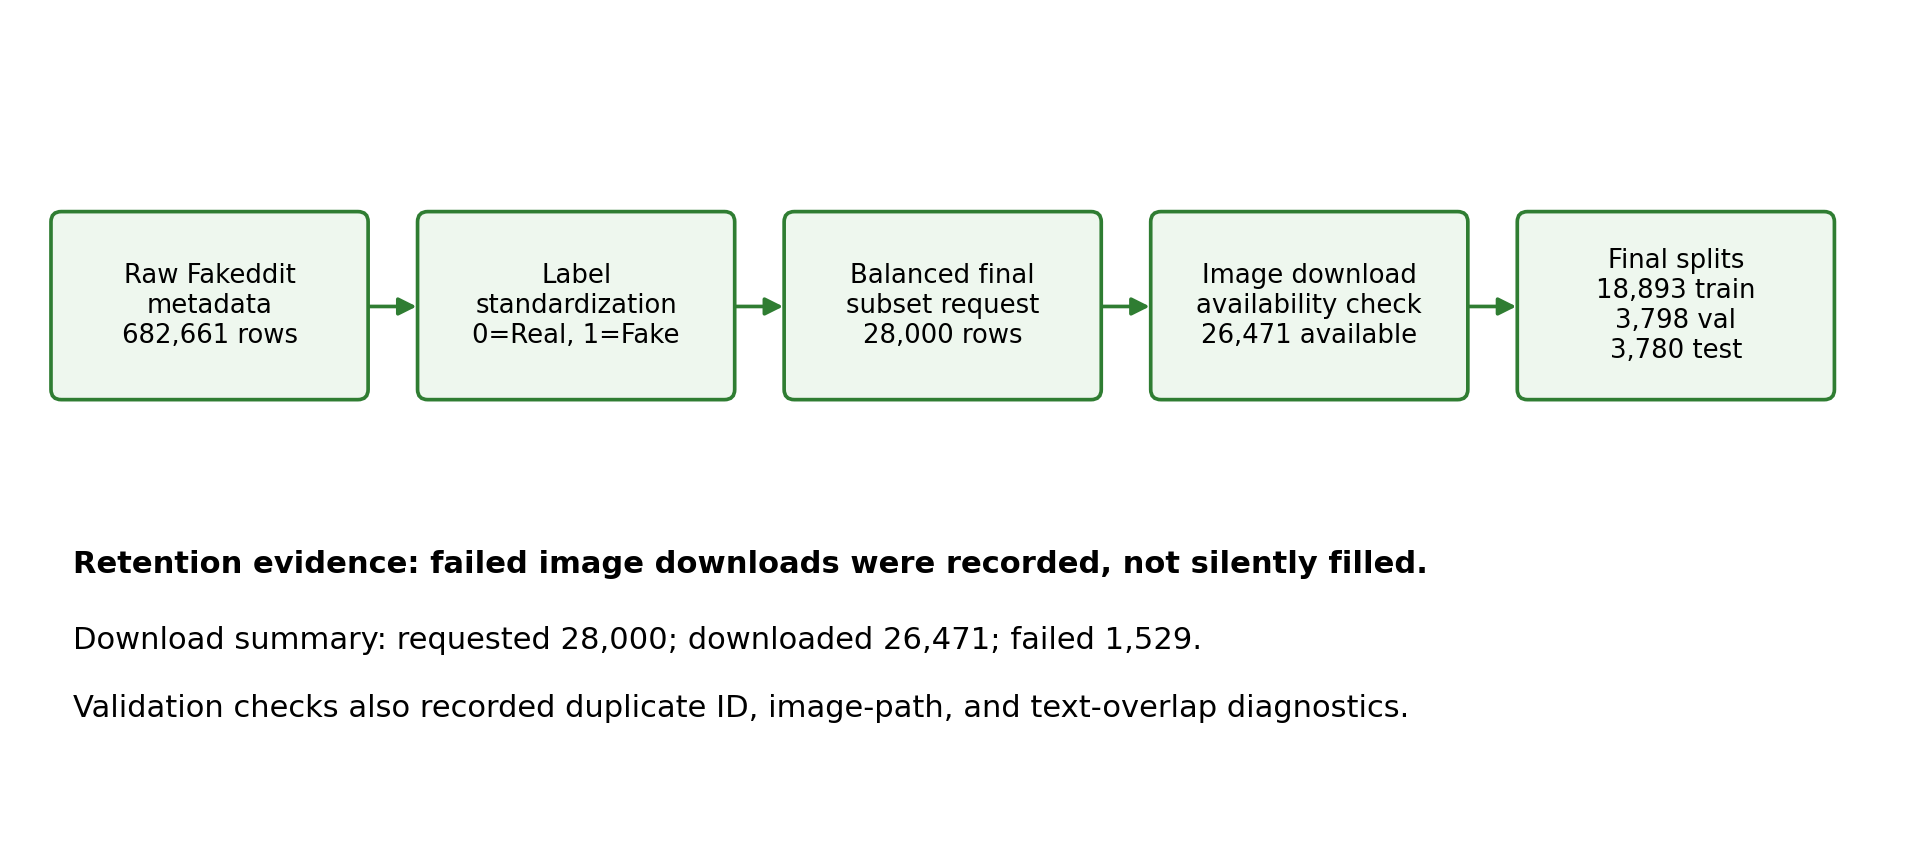
\includegraphics[width=0.92\textwidth,height=0.42\textheight,keepaspectratio]{figures/figure_5_2_data_preparation_and_retention.png}
\caption{Dataset preparation, image-availability filtering, and final split retention evidence.}
\label{fig:data_preparation_retention}
\end{figure}

The image reliability score is computed as the mean of availability and normalized visual quality cues:

\begin{equation}
q_i = \frac{q_{blur}+q_{brightness}+q_{contrast}+q_{entropy}+q_{available}}{5}
\label{eq:image_quality}
\end{equation}

The text reliability score is computed from length adequacy, truncation quality, and text availability:

\begin{equation}
q_t = \frac{q_{length}+q_{truncation}+q_{available}}{3}
\label{eq:text_quality}
\end{equation}

\clearpage
